%Code by K.A. Raja Babu
%May 15, 2021
%Constructing a quadrilateral PQRS
\documentclass[journal,12pt,twocolumn]{IEEEtran}

\usepackage{setspace}
\usepackage{gensymb}

\singlespacing


\usepackage[cmex10]{amsmath}

\usepackage{amsthm}

\usepackage{mathrsfs}
\usepackage{txfonts}
\usepackage{stfloats}
\usepackage{bm}
\usepackage{cite}
\usepackage{cases}
\usepackage{subfig}

\usepackage{longtable}
\usepackage{multirow}

\usepackage{enumitem}
\usepackage{mathtools}
\usepackage{steinmetz}
\usepackage{tikz}
\usepackage{circuitikz}
\usepackage{verbatim}
\usepackage{tfrupee}
\usepackage[breaklinks=true]{hyperref}
\usepackage{graphicx}
\usepackage{tkz-euclide}

\usetikzlibrary{calc,math}
\usepackage{listings}
    \usepackage{color}                                            %%
    \usepackage{array}                                            %%
    \usepackage{longtable}                                        %%
    \usepackage{calc}                                             %%
    \usepackage{multirow}                                         %%
    \usepackage{hhline}                                           %%
    \usepackage{ifthen}                                           %%
    \usepackage{lscape}     
\usepackage{multicol}
\usepackage{chngcntr}

\DeclareMathOperator*{\Res}{Res}

\renewcommand\thesection{\arabic{section}}
\renewcommand\thesubsection{\thesection.\arabic{subsection}}
\renewcommand\thesubsubsection{\thesubsection.\arabic{subsubsection}}

\renewcommand\thesectiondis{\arabic{section}}
\renewcommand\thesubsectiondis{\thesectiondis.\arabic{subsection}}
\renewcommand\thesubsubsectiondis{\thesubsectiondis.\arabic{subsubsection}}


\hyphenation{op-tical net-works semi-conduc-tor}
\def\inputGnumericTable{}                                 %%

\lstset{
%language=C,
frame=single, 
breaklines=true,
columns=fullflexible
}
\begin{document}

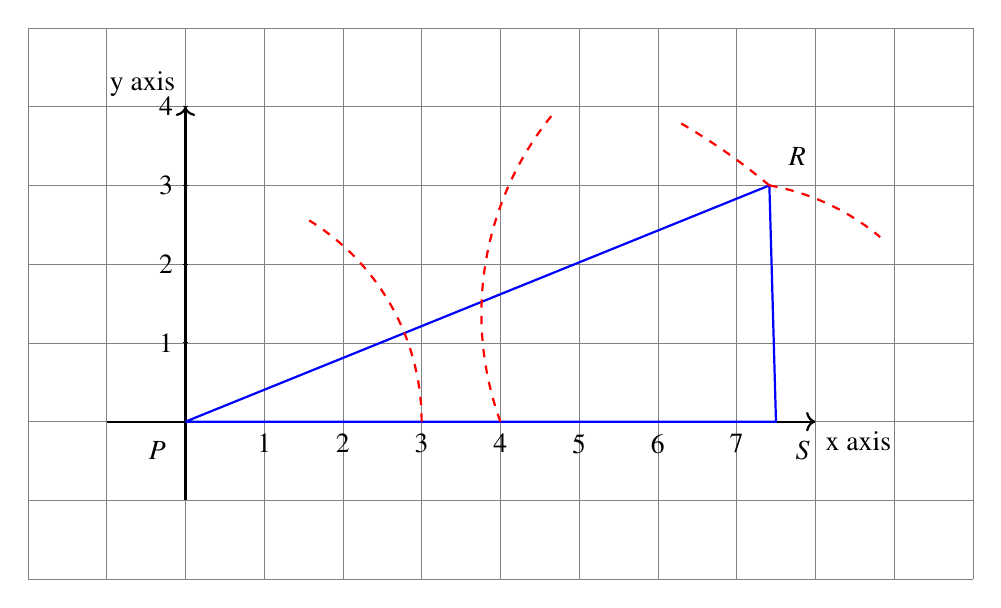
\begin{tikzpicture}
\centering
\draw[step=1cm,gray,very thin] (-2,-2) grid (10,5);

\draw[thick,->] (-1,0) -- (8,0) node[anchor=north west] {x axis};
\draw[thick,->] (0,-1) -- (0,4) node[anchor=south east] {y axis};

\foreach \x in {1,2,3,4,5,6,7}
   \draw (\x cm,-1pt) -- (\x cm,-1pt) node[anchor=north] {$\x$};
\foreach \y in {1,2,3,4}
    \draw (1pt,\y cm) -- (-1pt,\y cm) node[anchor=east] {$\y$};

\draw[blue,thick] (0,0)--(7.5,0)--(7.416,3)--(0,0);
\draw[red,thick,dashed] (7.416,3) arc (50:60:8cm);
\draw[red,thick,dashed] (7.416,3) arc (80:50:3cm);
\draw[red,thick,dashed] (3,0) arc (0:60:3cm);
\draw[red,thick,dashed] (4,0) arc (200:140:4cm);

%Labeling points
\node (P) at (0, 0)[label=below left:$P$] {};
\node (S) at (7.5, 0)[label=below right:$S$] {};
\node (R) at (7.416,3)[label=above right:$R$] {};
\end{tikzpicture}
\end{document}
